\subsection{Heurística Simmulated Annealing}

\subsubsection{El algoritmo}
Dada una función de distancia total, podemos calcular la utilidad de cada función, sabiendo que a menor distancia total, mejor es la solución. El dominio de esta función equivale a todas las solución posibles de de un problema de VRP, por lo que explorar la totalidad del dominio en busca del mínimo resulta inviable.

Sin embargo, partiendo de una solución aceptable encontrada por otra heurística, podemos tratar de explorar soluciones cercanas, en busca de hallar una mejor solución. Repitiendo este proceso buscamos minimizar la solución en función de la distancia total, llegando al mínimo global. Ver \textit{figura \ref{fig:convergencia}}

Para esto existe una gran cantidad de algoritmos, entre ellos:

\begin{itemize}\itemsep0em
\item Hill Climbing
\item Gradient Descent
\item Grasp
\item Tabu Search
\end{itemize}

Sin embargo, al hablar de VRP, nuestro dominio resulta ser más complejo, dando lugar a mínimos locales, en donde nuestro algoritmo puede quedar atrapado. Ver \textit{figura \ref{fig:minimo-local}}


\begin{figure}[H]
	\centering
	\begin{minipage}[t]{.45\textwidth}
		\centering
		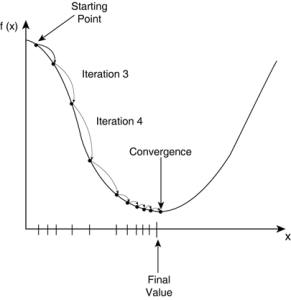
\includegraphics[scale=0.55]{annealing/fig1}
		\caption{Convergencia hacia el mínimo}
		\label{fig:convergencia}
	\end{minipage}\qquad
	\begin{minipage}[t]{.45\textwidth}
		\centering
		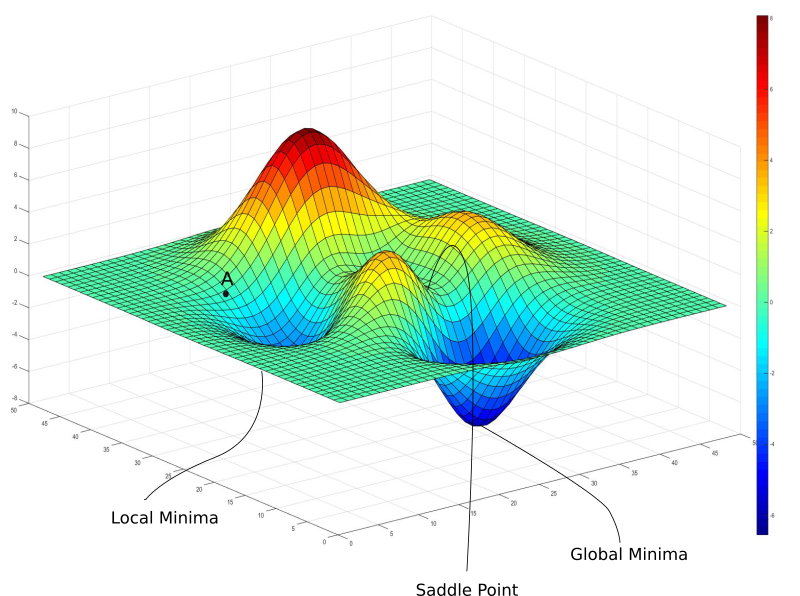
\includegraphics[scale=0.3]{annealing/fig2}
		\caption{Convergencia hacia el mínimo}
		\label{fig:minimo-local}
	\end{minipage}
\end{figure}	

Aquí es donde entra en escena Annealing, una metaheurística que trata de escaparse de los mínimos locales aceptando soluciones peores que la actual esperando desde esa peor solución llegar a una nueva que valga la pena.

El criterio que se utiliza para aceptar soluciones malas está basado en la práctica metalúrgica del recocido o \textbf{Anealing} en inglés.


Al moldear metales, se los calienta a temperaturas muy altas para poder ser moldeado, luego es enfriado para que vuelva a tomar las propiedades de rigidez y dureza. Algo parecido se busca obtener de la exploración de soluciones con está técnica.
Utilizando una temperatura artificial basada en propiedades de la solución vamos a definir cuán propensos somos a aceptar una solución mala, siguiendo el criterio de aceptar peores soluciones a mayor temperatura hasta gradualmente solo aceptar buenas soluciones una vez que nuestra temperatura se “enfríe”.


Existen múltiples versiones para la metaheurística de Annealing. a continuación presentamos el pseudocódigo para la versión reducida y la versión propuesta por Ibrahim Osman, la cual incluye resets de temperatura al llegar a caminos sin salida.

En general, las componentes comunes a las diferentes implementaciones de annealing son las siguientes:

\begin{itemize}
\item Función de energía: Define la calidad de la solución, cuanto menos tenga mejor. Se busca minimizar la energía.
\item Probabilidad de aceptación: Define la probabilidad de aceptar una solución propuesta, varía según la temperatura
\item Modificación de temperatura: Se aumenta o reduce la temperatura según la iteración y solución actual
\item Vecinos: La generación de soluciones vecinas depende del problema, se busca hacer modificaciones pequeñas.
\item Azar: Si bien utilizamos una función que nos devuelve la probabilidad de aceptar una solución, debemos comparar esa probabilidad contra un valor uniformemente aleatorio, esto significa que ejecutar el algoritmo con los mismos parámetros puede producir resultados diferentes.
\end{itemize}

\subsubsection{Pseudocodigo}

\begin{algorithm}[H]
\caption{Simple Simmulated Annealing}
\begin{algorithmic}[1]
\Function{Anneal}{Solucion $S_0$, Entero $T_{max}$, Entero $T_{min}$} 
\State $S \gets S_0$ 
\State $S_b \gets S_0$
\State $T \gets T_{max}$ 
\State
\While{$T > T_{min}$} 
	\State $S' \gets \textit{Vecino(S)}$
	\If{$\textit{ProbabilidadDeAceptar(S, S', T)} \geq \textit{Random(0, 1)} $}
		\State $S \gets S'$ 
	\EndIf	
	\State
	\If{$\textit{Energia(S)} < \textit{Energia}(S_b)$} 
		\State $S_b \gets S$ 
	\EndIf	
	\State \textit{Enfriar(T)} 
\EndWhile
\State
\State \Return $S_b$ 
\EndFunction
\end{algorithmic}
\end{algorithm}
\label{code:simple-annealing}

Como podemos ver, en esta versión de Annealing, establecemos un rango de temperaturas dentro del cual operar, explorando soluciones lindantes a la actual y aceptandolas de acuerdo a una probabilidad en función de la temperatura actual y la calidad de dicha solución.


Esto nos permite fácilmente tratar de minimizar nuestra solución inicial $S_0$, pero corremos el riesgo de quedar atrapados en un mínimo local según la probabilidad de aceptar una solución al azar.

Para combatir esto, decidimos seguir casi al pie de la letra la versión de Annealing descrita por \textit{Osman} en su paper, la cual al llegar a un camino sin salida, retrocede hasta la mejor solución encontrada, eleva la temperatura y prueba nuevamente de minimizar la solución, esperando esta vez seguir un camino diferente.


\begin{figure}[H]
	\centering
	\begin{minipage}[t]{.45\textwidth}
		\centering
		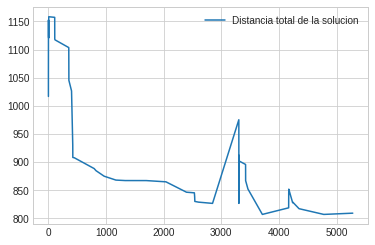
\includegraphics[scale=0.55]{annealing/distancia-total}
	\end{minipage}\qquad
	\begin{minipage}[t]{.45\textwidth}
		\centering
		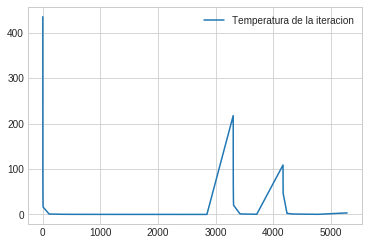
\includegraphics[scale=0.55]{annealing/temperatura}
	\end{minipage}
	
	Podemos ver como al elevarse la temperatura, se logra escapar de caminos sin salida, los cuales hubiesen sido devueltos como solución final por la implementación sencilla.
\end{figure}	


\begin{algorithm}[H]
\caption{Simmulated Annealing with Temperature Cycles}
\begin{algorithmic}[1]
\Function{Anneal}{Solucion $S_0$, Entero $R$} 
\State $S \gets S_0$ 
\State $S_b \gets S_0$ 
\State $T_s, T_f  \gets \textit{CalcularRangoDeTemperatura(S)}$
\State $T_k \gets T_{s}$ 
\State $resets \gets 0$ 
\State $k \gets 0$
\State
\While{$resets < R$} 
	\State $k \gets k + 1$ 
	\State
	\If{$\textit{HayVecinos(S)}$} 
		\State $\Delta_{energia} \gets \textit{ProximoVecino(S)}$ 
		\If{$\textit{ProbabilidadDeAceptar}(\Delta_{energia} , T_k) \geq \textit{Random(0, 1)} $} 
			\State $S \gets \textit{AceptarVecino(S)}$ 
		\EndIf
		\If{$\textit{Energia(S)} < \textit{Energia}(S_b)$}
			\State $S_b \gets S$ 
			\State $resets \gets 0$ 
		\EndIf	
		\State \textit{Enfriar($T_k$, $t_s$, $t_f$, $k$)}	
		\State
	\Else
		\State \textit{Calentar($T_k$, $t_s$, $t_f$, $k$)} 		
		\State $resets \gets resets + 1$ 
		\State \textit{GenerarNuevosVecinos(S)} 
	\EndIf

\EndWhile
\State
\State \Return $S_b$ 
\EndFunction
\end{algorithmic}
\end{algorithm}

Para poder entender el algoritmo, debemos conocer las siguientes funciones:

\begin{description}
\item[Energia] devuelve el la distancia total recorrida por los camiones en una solución, buscamos minimizarla

\item[CalcularRangoDeTemperatura] explora un vecindario completo de la solución y devuelve el mayor y menor cambio de energía encontrado

\item[HayVecinos] indica si quedan soluciones vecinas por explorar

\item[ProximoVecino] devuelve el la diferencia de energía entre la solución actual y el próximo vecino

\item[AceptarVecino] modifica la solución actual para reflejar el último vecino consultado

\item[ProbabilidadDeAceptar] dependiendo de la temperatura actual y la diferencia en energía propuesta, devuelve cierta probabilidad de que la solución sea aceptada (notar que el hecho de que sea aceptada o no, depende de que esta probabilidad sea mayor al número aleatorio contra el cual se compara) Esta sigue la fórmula:
$$ P = \mathlarger{\mathlarger{e^\frac{-\Delta_{energia}}{T_k}}} $$

\item[Enfriar] en base al rango de temperaturas de la solución inicial, la temperatura actual, iteración y otros parámetros, decrementa el valor de la temperatura actual, forzando a que la función “probabilidadDeAceptar” devuelva cada vez valores más bajos para una solución con un cambio de energía positivo (es decir, una solución peor a la actual)
esta sigue la formula: 
$$ T = \frac{T_k}{1+ \beta_k T_k},  \beta_k = \frac{T_s - T_f}{(\alpha + \gamma \sqrt{k} )T_s T_k} $$

\item[Calentar] eleva la temperatura actual a la temperatura que sea mayor entre la temperatura para la cual fue encontrada la mejor solución y la mitad de la temperatura del último reset

\item[NuevosVecinos] vuelve a recrear el vecindario de soluciones, para que pueda volver a ser explorado
\end{description}

Por ultimo, es necesario dar una explicación sobre la exploración del vecindario. Siguiendo lo propuesto por \textit{Ibrahim Osman}, utilizamos el metodo de exploracion Lambda-interchange para generar vecinos. Este método propone recorrer de manera aleatoria todas las combinaciones posibles entre camiones, y para cada una de ellas generar todos los intercambios posibles entre puntos según las siguientes operaciones.

Dadas dos rutas Rp y Rq, definimos:

\begin{description}
\item[Left shift:] Tomamos un punto de la ruta Rq y lo insertamos en la ruta Rq. está operación puede eliminar rutas

\item[Right shift:] Tomamos un punto de la ruta Rq y lo insertamos en la ruta Rp. está operación puede eliminar rutas

\item[Exchange:] Intercambiamos punto de la ruta Rq con uno de la ruta Rq
\end{description}

Esto nos permite generar un vecindario iterable de soluciones, el cual utilizamos para minimizar la energía.


\begin{figure}[H]
	\centering
	\begin{minipage}[t]{.3\textwidth}
		\centering
		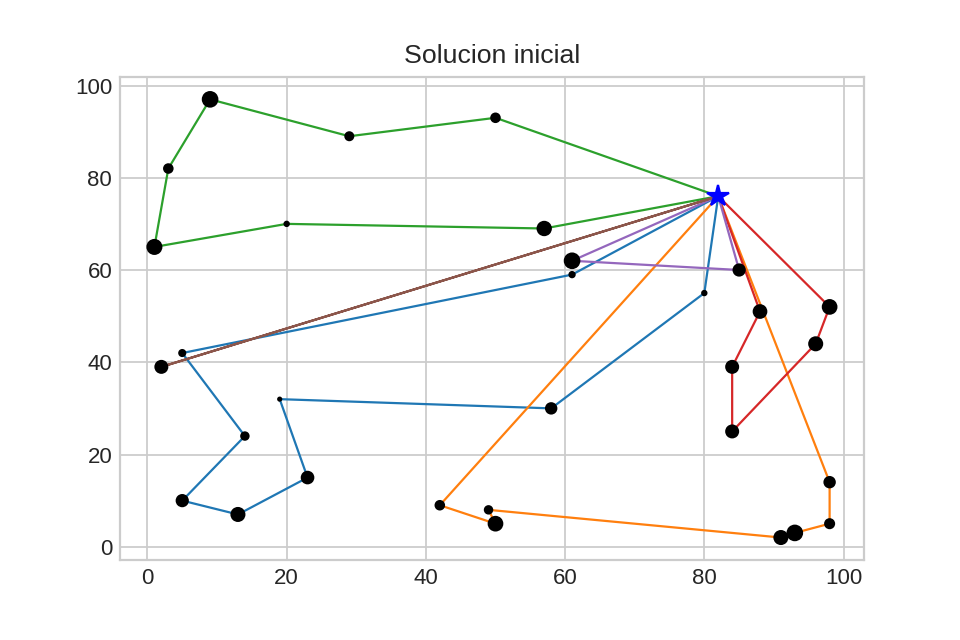
\includegraphics[scale=0.4]{annealing/exploracion-0}
	\end{minipage}\qquad
	\begin{minipage}[t]{.3\textwidth}
		\centering
		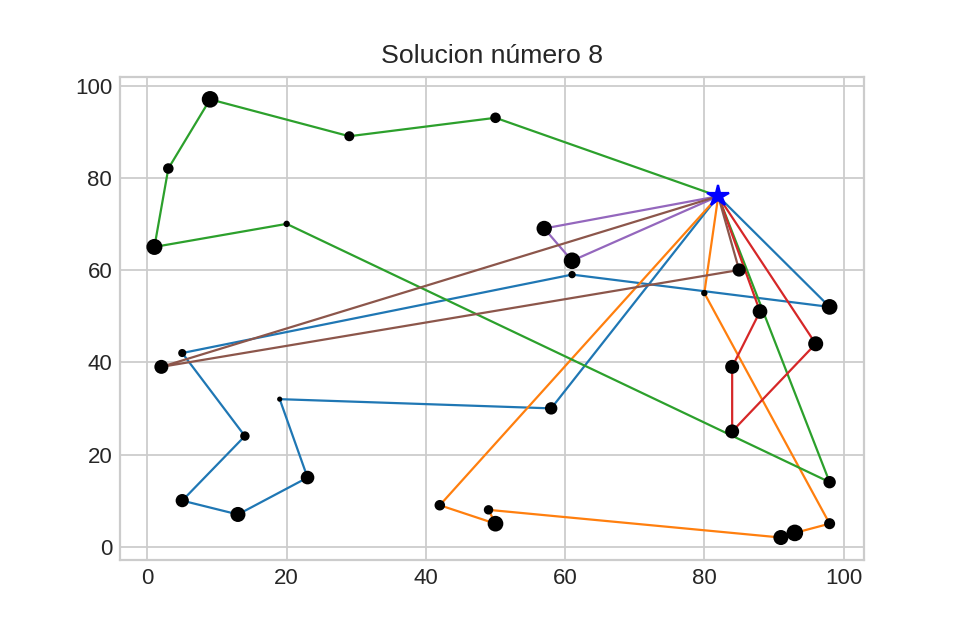
\includegraphics[scale=0.4]{annealing/exploracion-7}
	\end{minipage}\qquad
		\begin{minipage}[t]{.3\textwidth}
		\centering
		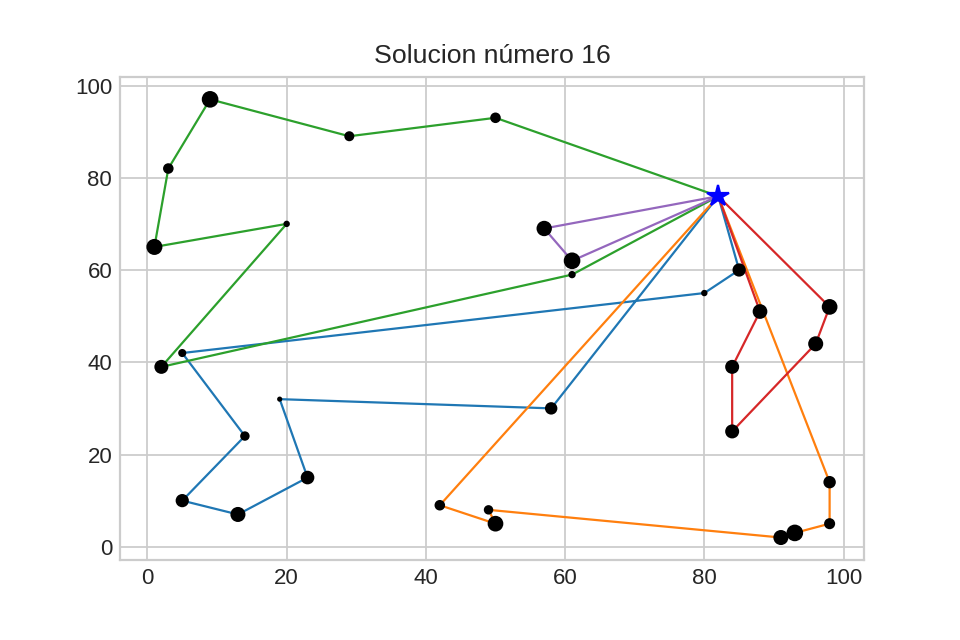
\includegraphics[scale=0.4]{annealing/exploracion-15}
	\end{minipage}\qquad
		\begin{minipage}[t]{.3\textwidth}
		\centering
		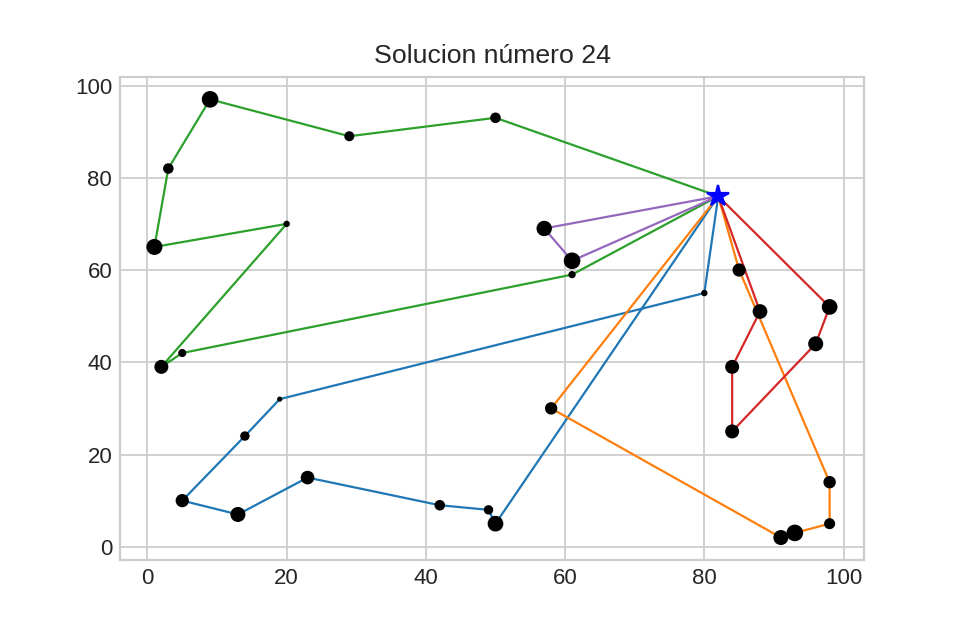
\includegraphics[scale=0.4]{annealing/exploracion-23}
	\end{minipage}\qquad
	\begin{minipage}[t]{.3\textwidth}
		\centering
		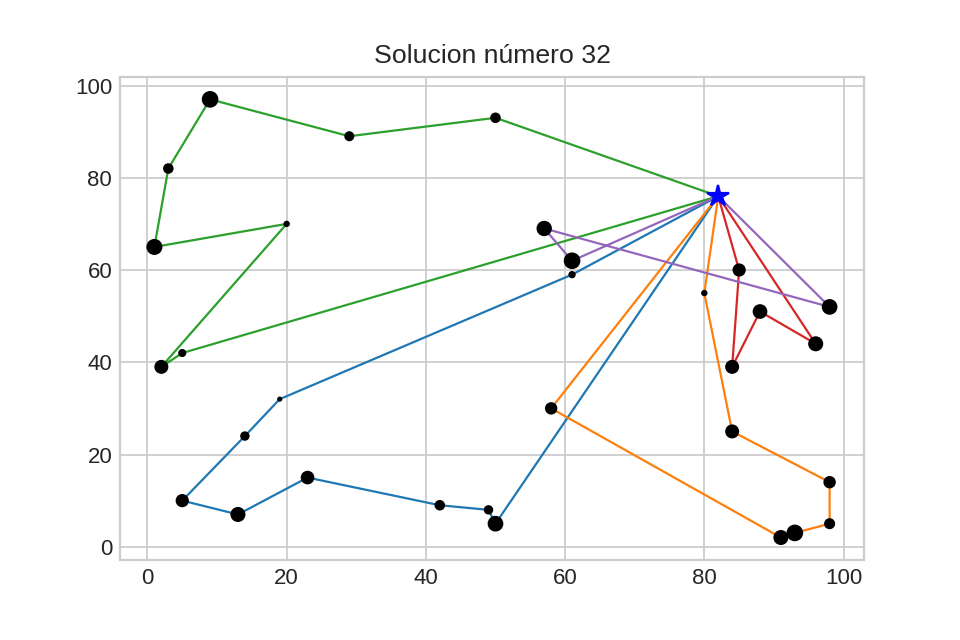
\includegraphics[scale=0.4]{annealing/exploracion-31}
	\end{minipage}\qquad
		\begin{minipage}[t]{.3\textwidth}
		\centering
		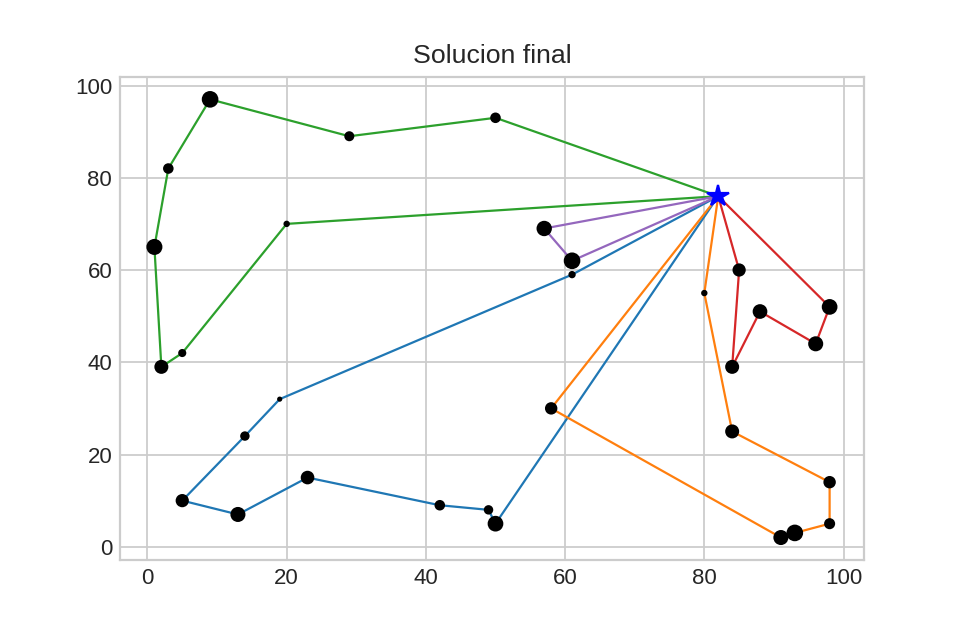
\includegraphics[scale=0.4]{annealing/exploracion-39}
	\end{minipage}\qquad
	
De solución inicial a final, en intervalos de a 8 exploraciones
\end{figure}


\subsubsection{Annealing en Accion}

A continuación podemos ver como tomando una solución de nuestra heurística golosa, Annealing trabaja para minimizar realizando varios ciclos de temperatura, escapando a mínimos locales y devolviendo una solución mucho más eficiente.

\begin{figure}[H]
	\centering
	\begin{minipage}[t]{.45\textwidth}
		\centering
		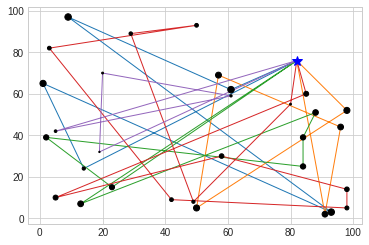
\includegraphics[scale=0.55]{annealing/greedy-inicio}
		\caption{Solucion inicial en base a Greedy}
	\end{minipage}\qquad
	\begin{minipage}[t]{.45\textwidth}
		\centering
		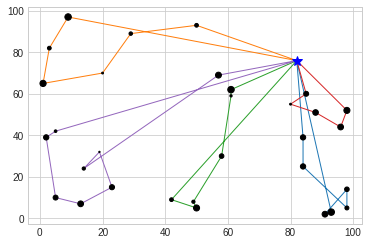
\includegraphics[scale=0.55]{annealing/greedy-final}
		\caption{Solucion final de Annealing}
	\end{minipage}
	
		\centering
	\begin{minipage}[t]{.45\textwidth}
		\centering
		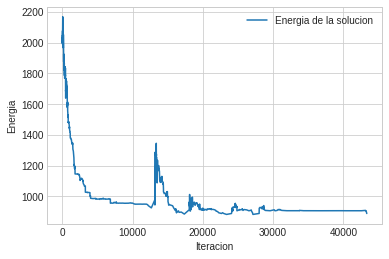
\includegraphics[scale=0.55]{annealing/greedy-energia}
		\caption{Energia de cada solucion}
	\end{minipage}\qquad
	\begin{minipage}[t]{.45\textwidth}
		\centering
		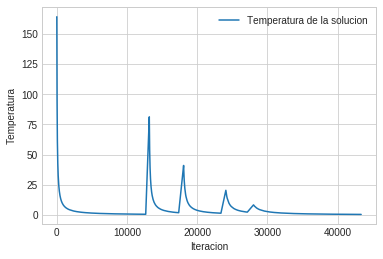
\includegraphics[scale=0.55]{annealing/greedy-temperatura}
		\caption{Temperatura en la iteracion}
	\end{minipage}
\end{figure}	

Podemos ver como para los primeros picos de temperatura (es decir, resets) el algorimo logra obtener una solucion mejor que la anterior, demostrando la utilidad de aceptar soluciones malas para escapar de optimos locales.



\subsubsection{Peores Casos}

La metaheurística de annealing se ve afectada por 3 factores que determinan qué tan probable es encontrar una solución óptima. Estos son la solución inicial, la forma del plano de la distancia total de las soluciones y el azar.

Annealing parte de una solución inicial ya calculada y de esta deriva la temperatura inicial y final por lo que cuando solución inicial es similar en energía a la solución óptima, puede resultar difícil hallar el camino entre las dos, dado que la temperatura no va a ser suficiente para escapar de los puntos silla.

\begin{figure}[H]
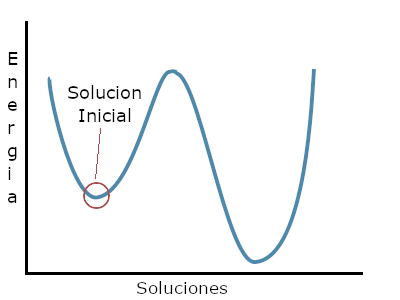
\includegraphics[scale=2]{annealing/mala-sol-inicial}
\centering
\end{figure}

Otro caso se basa en el mecanismo de exploración de vecindario, específicamente en las operaciones de intercambio. Cada camión tiene una capacidad máxima, por lo que no todas las operaciones se pueden aplicar para un conjunto de rutas y puntos.
Por ejemplo, si suponemos un camión sin capacidad disponible, entonces no va a ser posible realizar operaciones de shift que sumen puntos a su recorrido.
Un escenario complejo de este caso se da cuando no se puede realizar ninguna operación entre ningun camion, dado que cualquier punto intercambiado entre dos camiones excedería la capacidad de uno de los dos.
Si bien este escenario parece exagerado, es un escenario común (Probabilidad 1\%) para ciertos datasets particulares, o simplemente cuando el presupuesto de iteraciones para annealing es elevado.

\begin{figure}[H]
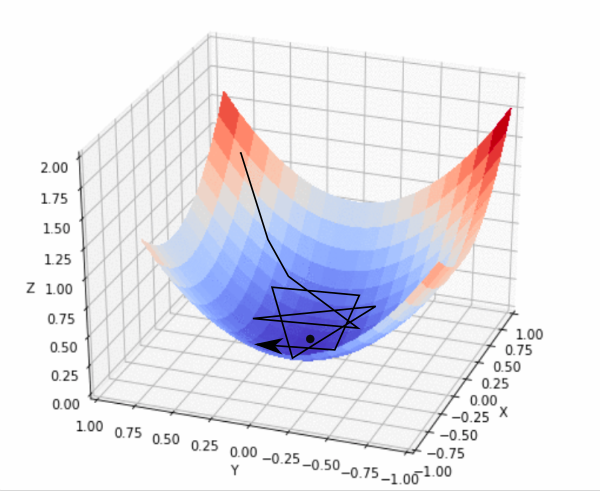
\includegraphics[scale=0.4]{annealing/rebote-convergencia}
\centering
\caption{Debido a baja temperatura y mala suerte, el algoritmo puede tardar en converger}

\end{figure}

\subsubsection{Complejidad}


Hablar sobre la complejidad de Simulated Annealing se torna difícil rápidamente, esto es porque a diferencia de algoritmos comunes, la continuación de la ejecución del mismo depende del camino actual tomado, la forma del plano de soluciones y lo más importante, el azar.

\vskip 1em

Si bien annealing utiliza una noción de temperatura inicial y final, no encontramos que en la versión propuesta por Ibrahim Osman en su paper \textit{Metastrategy simulated annealing and tabu search algorithms for the vehicle routing problem} que la temperatura actual alcance la final no es garantia de corte por varios motivos:
\begin{itemize}
\item Mientras se encuentren soluciones mejores que la actual, el algoritmo va a seguir explorando
\item No hay corte explícito por temperatura, solo por resets
\item Aun con una probabilidad muy baja de que una solución sea aceptada, igual puede pasar, lo cual prolonga la exploración.
\item Una vez que se llegó a un camino sin salida y se ejecuta un reset de temperatura, volvemos a tener la incertidumbre de cuando este va a converger.
\end{itemize}

Dado que evaluar el peor caso para el algoritmo no nos aporta ninguna información relevante, dado que nos encontraríamos con una cota masiva, decidimos evaluar la complejidad de la versión simple de Annealing (provista en \ref{code:simple-annealing}), es decir sin resets y con corte por temperatura, lo cual nos da una intuición de cómo se comporta la versión más compleja de Annealing.
\vskip 1em
En particular podemos ver que las complejidades que nos interesan averiguar son las de las funciones:
\begin{itemize}
\item Vecino
\item ProbabilidadDeAceptar
\item Energía
\item Enfriar
\end{itemize}

\begin{description}

\item[Vecino:] Como se explicó antes, para obtener el vecino de una solución, utilizamos el método de $\lambda$-interchange, el cual consiste en reemplazar, agregar o borrar puntos de una ruta.
Para realizar esto, es necesario recrear la ruta, dado que borrar un punto de un vector es una operación lineal (dado que se deben acomodar los elementos restantes). Luego, es necesario copiar esa solución para devolverla. Esto resulta en una función con complejidad lineal en base a la cantidad de puntos en el grafo. \textbf{Complejidad:} $\Theta(n)$ con n = cantidad de puntos

\item[Energía:] Se calcula la distancia total de una solución, para esto debemos recorrer la ruta propuesta en la solución, y hacer la suma de la distancia euclidiana entre los puntos. Dado que una solución pasa por todos los puntos (y no más de una vez),  tenemos a lo sumo $2*n$ operaciones. Donde $n$ es la cantidad total de puntos, y es multiplicada por 2 al tener en cuenta que el depósito está en cada ruta. \textbf{Complejidad}: $\Theta(n)$ con n = cantidad de puntos

\item[ProbabilidadDeAceptar:] Esta función tiene un costo constante, dado que se trata simplemente de una operación matemática (la cual fue explicada en la introducción a Annealing). Difiriendo con el pseudocódigo, elegimos pasar la energía de las soluciones en vez de las mismas, utilizandolas para la siguiente comparación. \textbf{Complejidad}: $\Theta(1)$

\item[Enfriar:] Esta función tiene un costo constante, dado que se trata simplemente de una operación matemática (la cual fue explicada en la introducción a Annealing). \textbf{Complejidad}: $\Theta(1)$

\end{description}

Respecto al pseudocódigo de Annealing con resets, se agregan las siguientes funciones:

\begin{description}

\item[HayVecinos:] Se utilizan iteradores para saber si hay mas rutas para comparar. \textbf{Complejidad}: $\Theta(1)$

\item[ProximoVecino:] Igual que Vecino, pero devuelve el cálculo de energía.  \textbf{Complejidad}: $\Theta(n)$ con n = cantidad de puntos

\item[AceptarVecino:] Simplemente devuelve por referencia la solución anteriormente generada y guardada en una variable.  \textbf{Complejidad}: $\Theta(1)$

\item[GenerarNuevosVecinos:] Se vuelven a inicializar los iteradores que apuntan a las rutas a comparar. \textbf{Complejidad}: $\Theta(1)$

\item[Calentar:] Esta función tiene un costo constante, dado que se trata simplemente de una operación matemática (la cual fue explicada en la introducción a Annealing). \textbf{Complejidad}: $\Theta(1)$

\end{description}

Respecto a la cuenta de enfriamiento temperatura, vamos a utilizar la que describimos anteriormente en la introducción, es decir 
$$ T = \frac{T_k}{1+ \beta_k T_k},  \beta_k = \frac{T_s - T_f}{(\alpha + \gamma \sqrt{k} )T_s T_k} $$

\vskip 1em
Donde 
\begin{description}
\item[$\alpha$ = ] cantidad de puntos * constante
\item[$\sigma$ = ] cantidad de puntos
\item[K = ] iteracion actual
\end{description}


\begin{figure}[H]
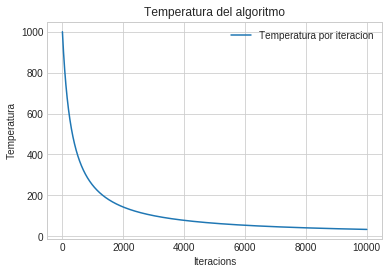
\includegraphics[scale=0.4]{annealing/complejidad}
\centering
\caption{La temperatura en base a las iteraciones}

\end{figure}

Al graficar la función, podemos ver como converge rápidamente, tomando unas 10000 iteraciones para llevar la temperatura actual a la final (con $t_s = 1000$, $t_f = 10$, $n = 32$, $\alpha = n * 1000$). Luego podemos deducir que existe un valor $iteraciones_{temp}$ en base a $n$ para la cual cualquier configuracion de parametros va a converger.
\vskip 1em
Luego podemos definir la complejidad como $\Theta(n * iteraciones_{temp})$





\section{Experimentación}

\subsection{Aclaraciones}

Para la siguiente experimentación, se optó por tomar dos casos distintos para graficar la performance de cada heurística:

\begin{itemize}
\item Medición de performance en base a tamaño del grafo.
\item Medición de performance en base a distribución del grafo.
\end{itemize}

\subsubsection{Medición en base a tamaño del grafo}
Para realizar el siguiente experimento, se tomaron datasets con distintas distribuciones del mismo tamaño y se tomó el promedio de ejecución para cada uno de ellos en base a 50 ejecuciones. En base a los resultados obtenidos, se seleccionó el mejor caso y se realizaron pruebas sobre datasets incrementando el tamaño.

\vskip 8pt

El punto de partida es un dataset de tamaño n = 45 ya que dicho tamaño se encontraba disponible para todos los tipos de datasets a experimentar.

\subsubsection{Medición en base a tamaño del grafo}
En base al mejor caso encontrado para el punto anterior, se utilizaron las demás instancias para mostrar como la distribución del grafo afecta la performance del mismo.

\section{Experimentación}

\subsection{Aclaraciones}

Para la siguiente experimentación, se optó por tomar dos casos distintos para graficar la performance de cada heurística:

\begin{itemize}
\item Medición de performance en base a tamaño del grafo.
\item Medición de performance en base a distribución del grafo.
\end{itemize}

\subsubsection{Medición en base a tamaño del grafo}
Para realizar el siguiente experimento, se tomaron datasets con distintas distribuciones del mismo tamaño y se tomó el promedio de ejecución para cada uno de ellos en base a 50 ejecuciones. En base a los resultados obtenidos, se seleccionó el mejor caso y se realizaron pruebas sobre datasets incrementando el tamaño.

\vskip 8pt

El punto de partida es un dataset de tamaño n = 45 ya que dicho tamaño se encontraba disponible para todos los tipos de datasets a experimentar.

\subsubsection{Medición en base a tamaño del grafo}
En base al mejor caso encontrado para el punto anterior, se utilizaron las demás instancias para mostrar como la distribución del grafo afecta la performance del mismo.

\section{Experimentación}

\subsection{Aclaraciones}

Para la siguiente experimentación, se optó por tomar dos casos distintos para graficar la performance de cada heurística:

\begin{itemize}
\item Medición de performance en base a tamaño del grafo.
\item Medición de performance en base a distribución del grafo.
\end{itemize}

\subsubsection{Medición en base a tamaño del grafo}
Para realizar el siguiente experimento, se tomaron datasets con distintas distribuciones del mismo tamaño y se tomó el promedio de ejecución para cada uno de ellos en base a 50 ejecuciones. En base a los resultados obtenidos, se seleccionó el mejor caso y se realizaron pruebas sobre datasets incrementando el tamaño.

\vskip 8pt

El punto de partida es un dataset de tamaño n = 45 ya que dicho tamaño se encontraba disponible para todos los tipos de datasets a experimentar.

\subsubsection{Medición en base a tamaño del grafo}
En base al mejor caso encontrado para el punto anterior, se utilizaron las demás instancias para mostrar como la distribución del grafo afecta la performance del mismo.

\input{sections/savings/experimentacion}
\input{sections/greedy/experimentacion}
\input{sections/sweep/experimentacion}
\input{sections/kmeans/experimentacion}
\input{sections/annealing/experimentacion}


\section{Experimentación}

\subsection{Aclaraciones}

Para la siguiente experimentación, se optó por tomar dos casos distintos para graficar la performance de cada heurística:

\begin{itemize}
\item Medición de performance en base a tamaño del grafo.
\item Medición de performance en base a distribución del grafo.
\end{itemize}

\subsubsection{Medición en base a tamaño del grafo}
Para realizar el siguiente experimento, se tomaron datasets con distintas distribuciones del mismo tamaño y se tomó el promedio de ejecución para cada uno de ellos en base a 50 ejecuciones. En base a los resultados obtenidos, se seleccionó el mejor caso y se realizaron pruebas sobre datasets incrementando el tamaño.

\vskip 8pt

El punto de partida es un dataset de tamaño n = 45 ya que dicho tamaño se encontraba disponible para todos los tipos de datasets a experimentar.

\subsubsection{Medición en base a tamaño del grafo}
En base al mejor caso encontrado para el punto anterior, se utilizaron las demás instancias para mostrar como la distribución del grafo afecta la performance del mismo.

\input{sections/savings/experimentacion}
\input{sections/greedy/experimentacion}
\input{sections/sweep/experimentacion}
\input{sections/kmeans/experimentacion}
\input{sections/annealing/experimentacion}


\section{Experimentación}

\subsection{Aclaraciones}

Para la siguiente experimentación, se optó por tomar dos casos distintos para graficar la performance de cada heurística:

\begin{itemize}
\item Medición de performance en base a tamaño del grafo.
\item Medición de performance en base a distribución del grafo.
\end{itemize}

\subsubsection{Medición en base a tamaño del grafo}
Para realizar el siguiente experimento, se tomaron datasets con distintas distribuciones del mismo tamaño y se tomó el promedio de ejecución para cada uno de ellos en base a 50 ejecuciones. En base a los resultados obtenidos, se seleccionó el mejor caso y se realizaron pruebas sobre datasets incrementando el tamaño.

\vskip 8pt

El punto de partida es un dataset de tamaño n = 45 ya que dicho tamaño se encontraba disponible para todos los tipos de datasets a experimentar.

\subsubsection{Medición en base a tamaño del grafo}
En base al mejor caso encontrado para el punto anterior, se utilizaron las demás instancias para mostrar como la distribución del grafo afecta la performance del mismo.

\input{sections/savings/experimentacion}
\input{sections/greedy/experimentacion}
\input{sections/sweep/experimentacion}
\input{sections/kmeans/experimentacion}
\input{sections/annealing/experimentacion}


\section{Experimentación}

\subsection{Aclaraciones}

Para la siguiente experimentación, se optó por tomar dos casos distintos para graficar la performance de cada heurística:

\begin{itemize}
\item Medición de performance en base a tamaño del grafo.
\item Medición de performance en base a distribución del grafo.
\end{itemize}

\subsubsection{Medición en base a tamaño del grafo}
Para realizar el siguiente experimento, se tomaron datasets con distintas distribuciones del mismo tamaño y se tomó el promedio de ejecución para cada uno de ellos en base a 50 ejecuciones. En base a los resultados obtenidos, se seleccionó el mejor caso y se realizaron pruebas sobre datasets incrementando el tamaño.

\vskip 8pt

El punto de partida es un dataset de tamaño n = 45 ya que dicho tamaño se encontraba disponible para todos los tipos de datasets a experimentar.

\subsubsection{Medición en base a tamaño del grafo}
En base al mejor caso encontrado para el punto anterior, se utilizaron las demás instancias para mostrar como la distribución del grafo afecta la performance del mismo.

\input{sections/savings/experimentacion}
\input{sections/greedy/experimentacion}
\input{sections/sweep/experimentacion}
\input{sections/kmeans/experimentacion}
\input{sections/annealing/experimentacion}


\section{Experimentación}

\subsection{Aclaraciones}

Para la siguiente experimentación, se optó por tomar dos casos distintos para graficar la performance de cada heurística:

\begin{itemize}
\item Medición de performance en base a tamaño del grafo.
\item Medición de performance en base a distribución del grafo.
\end{itemize}

\subsubsection{Medición en base a tamaño del grafo}
Para realizar el siguiente experimento, se tomaron datasets con distintas distribuciones del mismo tamaño y se tomó el promedio de ejecución para cada uno de ellos en base a 50 ejecuciones. En base a los resultados obtenidos, se seleccionó el mejor caso y se realizaron pruebas sobre datasets incrementando el tamaño.

\vskip 8pt

El punto de partida es un dataset de tamaño n = 45 ya que dicho tamaño se encontraba disponible para todos los tipos de datasets a experimentar.

\subsubsection{Medición en base a tamaño del grafo}
En base al mejor caso encontrado para el punto anterior, se utilizaron las demás instancias para mostrar como la distribución del grafo afecta la performance del mismo.

\input{sections/savings/experimentacion}
\input{sections/greedy/experimentacion}
\input{sections/sweep/experimentacion}
\input{sections/kmeans/experimentacion}
\input{sections/annealing/experimentacion}




\section{Experimentación}

\subsection{Aclaraciones}

Para la siguiente experimentación, se optó por tomar dos casos distintos para graficar la performance de cada heurística:

\begin{itemize}
\item Medición de performance en base a tamaño del grafo.
\item Medición de performance en base a distribución del grafo.
\end{itemize}

\subsubsection{Medición en base a tamaño del grafo}
Para realizar el siguiente experimento, se tomaron datasets con distintas distribuciones del mismo tamaño y se tomó el promedio de ejecución para cada uno de ellos en base a 50 ejecuciones. En base a los resultados obtenidos, se seleccionó el mejor caso y se realizaron pruebas sobre datasets incrementando el tamaño.

\vskip 8pt

El punto de partida es un dataset de tamaño n = 45 ya que dicho tamaño se encontraba disponible para todos los tipos de datasets a experimentar.

\subsubsection{Medición en base a tamaño del grafo}
En base al mejor caso encontrado para el punto anterior, se utilizaron las demás instancias para mostrar como la distribución del grafo afecta la performance del mismo.

\section{Experimentación}

\subsection{Aclaraciones}

Para la siguiente experimentación, se optó por tomar dos casos distintos para graficar la performance de cada heurística:

\begin{itemize}
\item Medición de performance en base a tamaño del grafo.
\item Medición de performance en base a distribución del grafo.
\end{itemize}

\subsubsection{Medición en base a tamaño del grafo}
Para realizar el siguiente experimento, se tomaron datasets con distintas distribuciones del mismo tamaño y se tomó el promedio de ejecución para cada uno de ellos en base a 50 ejecuciones. En base a los resultados obtenidos, se seleccionó el mejor caso y se realizaron pruebas sobre datasets incrementando el tamaño.

\vskip 8pt

El punto de partida es un dataset de tamaño n = 45 ya que dicho tamaño se encontraba disponible para todos los tipos de datasets a experimentar.

\subsubsection{Medición en base a tamaño del grafo}
En base al mejor caso encontrado para el punto anterior, se utilizaron las demás instancias para mostrar como la distribución del grafo afecta la performance del mismo.

\input{sections/savings/experimentacion}
\input{sections/greedy/experimentacion}
\input{sections/sweep/experimentacion}
\input{sections/kmeans/experimentacion}
\input{sections/annealing/experimentacion}


\section{Experimentación}

\subsection{Aclaraciones}

Para la siguiente experimentación, se optó por tomar dos casos distintos para graficar la performance de cada heurística:

\begin{itemize}
\item Medición de performance en base a tamaño del grafo.
\item Medición de performance en base a distribución del grafo.
\end{itemize}

\subsubsection{Medición en base a tamaño del grafo}
Para realizar el siguiente experimento, se tomaron datasets con distintas distribuciones del mismo tamaño y se tomó el promedio de ejecución para cada uno de ellos en base a 50 ejecuciones. En base a los resultados obtenidos, se seleccionó el mejor caso y se realizaron pruebas sobre datasets incrementando el tamaño.

\vskip 8pt

El punto de partida es un dataset de tamaño n = 45 ya que dicho tamaño se encontraba disponible para todos los tipos de datasets a experimentar.

\subsubsection{Medición en base a tamaño del grafo}
En base al mejor caso encontrado para el punto anterior, se utilizaron las demás instancias para mostrar como la distribución del grafo afecta la performance del mismo.

\input{sections/savings/experimentacion}
\input{sections/greedy/experimentacion}
\input{sections/sweep/experimentacion}
\input{sections/kmeans/experimentacion}
\input{sections/annealing/experimentacion}


\section{Experimentación}

\subsection{Aclaraciones}

Para la siguiente experimentación, se optó por tomar dos casos distintos para graficar la performance de cada heurística:

\begin{itemize}
\item Medición de performance en base a tamaño del grafo.
\item Medición de performance en base a distribución del grafo.
\end{itemize}

\subsubsection{Medición en base a tamaño del grafo}
Para realizar el siguiente experimento, se tomaron datasets con distintas distribuciones del mismo tamaño y se tomó el promedio de ejecución para cada uno de ellos en base a 50 ejecuciones. En base a los resultados obtenidos, se seleccionó el mejor caso y se realizaron pruebas sobre datasets incrementando el tamaño.

\vskip 8pt

El punto de partida es un dataset de tamaño n = 45 ya que dicho tamaño se encontraba disponible para todos los tipos de datasets a experimentar.

\subsubsection{Medición en base a tamaño del grafo}
En base al mejor caso encontrado para el punto anterior, se utilizaron las demás instancias para mostrar como la distribución del grafo afecta la performance del mismo.

\input{sections/savings/experimentacion}
\input{sections/greedy/experimentacion}
\input{sections/sweep/experimentacion}
\input{sections/kmeans/experimentacion}
\input{sections/annealing/experimentacion}


\section{Experimentación}

\subsection{Aclaraciones}

Para la siguiente experimentación, se optó por tomar dos casos distintos para graficar la performance de cada heurística:

\begin{itemize}
\item Medición de performance en base a tamaño del grafo.
\item Medición de performance en base a distribución del grafo.
\end{itemize}

\subsubsection{Medición en base a tamaño del grafo}
Para realizar el siguiente experimento, se tomaron datasets con distintas distribuciones del mismo tamaño y se tomó el promedio de ejecución para cada uno de ellos en base a 50 ejecuciones. En base a los resultados obtenidos, se seleccionó el mejor caso y se realizaron pruebas sobre datasets incrementando el tamaño.

\vskip 8pt

El punto de partida es un dataset de tamaño n = 45 ya que dicho tamaño se encontraba disponible para todos los tipos de datasets a experimentar.

\subsubsection{Medición en base a tamaño del grafo}
En base al mejor caso encontrado para el punto anterior, se utilizaron las demás instancias para mostrar como la distribución del grafo afecta la performance del mismo.

\input{sections/savings/experimentacion}
\input{sections/greedy/experimentacion}
\input{sections/sweep/experimentacion}
\input{sections/kmeans/experimentacion}
\input{sections/annealing/experimentacion}


\section{Experimentación}

\subsection{Aclaraciones}

Para la siguiente experimentación, se optó por tomar dos casos distintos para graficar la performance de cada heurística:

\begin{itemize}
\item Medición de performance en base a tamaño del grafo.
\item Medición de performance en base a distribución del grafo.
\end{itemize}

\subsubsection{Medición en base a tamaño del grafo}
Para realizar el siguiente experimento, se tomaron datasets con distintas distribuciones del mismo tamaño y se tomó el promedio de ejecución para cada uno de ellos en base a 50 ejecuciones. En base a los resultados obtenidos, se seleccionó el mejor caso y se realizaron pruebas sobre datasets incrementando el tamaño.

\vskip 8pt

El punto de partida es un dataset de tamaño n = 45 ya que dicho tamaño se encontraba disponible para todos los tipos de datasets a experimentar.

\subsubsection{Medición en base a tamaño del grafo}
En base al mejor caso encontrado para el punto anterior, se utilizaron las demás instancias para mostrar como la distribución del grafo afecta la performance del mismo.

\input{sections/savings/experimentacion}
\input{sections/greedy/experimentacion}
\input{sections/sweep/experimentacion}
\input{sections/kmeans/experimentacion}
\input{sections/annealing/experimentacion}




\section{Experimentación}

\subsection{Aclaraciones}

Para la siguiente experimentación, se optó por tomar dos casos distintos para graficar la performance de cada heurística:

\begin{itemize}
\item Medición de performance en base a tamaño del grafo.
\item Medición de performance en base a distribución del grafo.
\end{itemize}

\subsubsection{Medición en base a tamaño del grafo}
Para realizar el siguiente experimento, se tomaron datasets con distintas distribuciones del mismo tamaño y se tomó el promedio de ejecución para cada uno de ellos en base a 50 ejecuciones. En base a los resultados obtenidos, se seleccionó el mejor caso y se realizaron pruebas sobre datasets incrementando el tamaño.

\vskip 8pt

El punto de partida es un dataset de tamaño n = 45 ya que dicho tamaño se encontraba disponible para todos los tipos de datasets a experimentar.

\subsubsection{Medición en base a tamaño del grafo}
En base al mejor caso encontrado para el punto anterior, se utilizaron las demás instancias para mostrar como la distribución del grafo afecta la performance del mismo.

\section{Experimentación}

\subsection{Aclaraciones}

Para la siguiente experimentación, se optó por tomar dos casos distintos para graficar la performance de cada heurística:

\begin{itemize}
\item Medición de performance en base a tamaño del grafo.
\item Medición de performance en base a distribución del grafo.
\end{itemize}

\subsubsection{Medición en base a tamaño del grafo}
Para realizar el siguiente experimento, se tomaron datasets con distintas distribuciones del mismo tamaño y se tomó el promedio de ejecución para cada uno de ellos en base a 50 ejecuciones. En base a los resultados obtenidos, se seleccionó el mejor caso y se realizaron pruebas sobre datasets incrementando el tamaño.

\vskip 8pt

El punto de partida es un dataset de tamaño n = 45 ya que dicho tamaño se encontraba disponible para todos los tipos de datasets a experimentar.

\subsubsection{Medición en base a tamaño del grafo}
En base al mejor caso encontrado para el punto anterior, se utilizaron las demás instancias para mostrar como la distribución del grafo afecta la performance del mismo.

\input{sections/savings/experimentacion}
\input{sections/greedy/experimentacion}
\input{sections/sweep/experimentacion}
\input{sections/kmeans/experimentacion}
\input{sections/annealing/experimentacion}


\section{Experimentación}

\subsection{Aclaraciones}

Para la siguiente experimentación, se optó por tomar dos casos distintos para graficar la performance de cada heurística:

\begin{itemize}
\item Medición de performance en base a tamaño del grafo.
\item Medición de performance en base a distribución del grafo.
\end{itemize}

\subsubsection{Medición en base a tamaño del grafo}
Para realizar el siguiente experimento, se tomaron datasets con distintas distribuciones del mismo tamaño y se tomó el promedio de ejecución para cada uno de ellos en base a 50 ejecuciones. En base a los resultados obtenidos, se seleccionó el mejor caso y se realizaron pruebas sobre datasets incrementando el tamaño.

\vskip 8pt

El punto de partida es un dataset de tamaño n = 45 ya que dicho tamaño se encontraba disponible para todos los tipos de datasets a experimentar.

\subsubsection{Medición en base a tamaño del grafo}
En base al mejor caso encontrado para el punto anterior, se utilizaron las demás instancias para mostrar como la distribución del grafo afecta la performance del mismo.

\input{sections/savings/experimentacion}
\input{sections/greedy/experimentacion}
\input{sections/sweep/experimentacion}
\input{sections/kmeans/experimentacion}
\input{sections/annealing/experimentacion}


\section{Experimentación}

\subsection{Aclaraciones}

Para la siguiente experimentación, se optó por tomar dos casos distintos para graficar la performance de cada heurística:

\begin{itemize}
\item Medición de performance en base a tamaño del grafo.
\item Medición de performance en base a distribución del grafo.
\end{itemize}

\subsubsection{Medición en base a tamaño del grafo}
Para realizar el siguiente experimento, se tomaron datasets con distintas distribuciones del mismo tamaño y se tomó el promedio de ejecución para cada uno de ellos en base a 50 ejecuciones. En base a los resultados obtenidos, se seleccionó el mejor caso y se realizaron pruebas sobre datasets incrementando el tamaño.

\vskip 8pt

El punto de partida es un dataset de tamaño n = 45 ya que dicho tamaño se encontraba disponible para todos los tipos de datasets a experimentar.

\subsubsection{Medición en base a tamaño del grafo}
En base al mejor caso encontrado para el punto anterior, se utilizaron las demás instancias para mostrar como la distribución del grafo afecta la performance del mismo.

\input{sections/savings/experimentacion}
\input{sections/greedy/experimentacion}
\input{sections/sweep/experimentacion}
\input{sections/kmeans/experimentacion}
\input{sections/annealing/experimentacion}


\section{Experimentación}

\subsection{Aclaraciones}

Para la siguiente experimentación, se optó por tomar dos casos distintos para graficar la performance de cada heurística:

\begin{itemize}
\item Medición de performance en base a tamaño del grafo.
\item Medición de performance en base a distribución del grafo.
\end{itemize}

\subsubsection{Medición en base a tamaño del grafo}
Para realizar el siguiente experimento, se tomaron datasets con distintas distribuciones del mismo tamaño y se tomó el promedio de ejecución para cada uno de ellos en base a 50 ejecuciones. En base a los resultados obtenidos, se seleccionó el mejor caso y se realizaron pruebas sobre datasets incrementando el tamaño.

\vskip 8pt

El punto de partida es un dataset de tamaño n = 45 ya que dicho tamaño se encontraba disponible para todos los tipos de datasets a experimentar.

\subsubsection{Medición en base a tamaño del grafo}
En base al mejor caso encontrado para el punto anterior, se utilizaron las demás instancias para mostrar como la distribución del grafo afecta la performance del mismo.

\input{sections/savings/experimentacion}
\input{sections/greedy/experimentacion}
\input{sections/sweep/experimentacion}
\input{sections/kmeans/experimentacion}
\input{sections/annealing/experimentacion}


\section{Experimentación}

\subsection{Aclaraciones}

Para la siguiente experimentación, se optó por tomar dos casos distintos para graficar la performance de cada heurística:

\begin{itemize}
\item Medición de performance en base a tamaño del grafo.
\item Medición de performance en base a distribución del grafo.
\end{itemize}

\subsubsection{Medición en base a tamaño del grafo}
Para realizar el siguiente experimento, se tomaron datasets con distintas distribuciones del mismo tamaño y se tomó el promedio de ejecución para cada uno de ellos en base a 50 ejecuciones. En base a los resultados obtenidos, se seleccionó el mejor caso y se realizaron pruebas sobre datasets incrementando el tamaño.

\vskip 8pt

El punto de partida es un dataset de tamaño n = 45 ya que dicho tamaño se encontraba disponible para todos los tipos de datasets a experimentar.

\subsubsection{Medición en base a tamaño del grafo}
En base al mejor caso encontrado para el punto anterior, se utilizaron las demás instancias para mostrar como la distribución del grafo afecta la performance del mismo.

\input{sections/savings/experimentacion}
\input{sections/greedy/experimentacion}
\input{sections/sweep/experimentacion}
\input{sections/kmeans/experimentacion}
\input{sections/annealing/experimentacion}




\section{Experimentación}

\subsection{Aclaraciones}

Para la siguiente experimentación, se optó por tomar dos casos distintos para graficar la performance de cada heurística:

\begin{itemize}
\item Medición de performance en base a tamaño del grafo.
\item Medición de performance en base a distribución del grafo.
\end{itemize}

\subsubsection{Medición en base a tamaño del grafo}
Para realizar el siguiente experimento, se tomaron datasets con distintas distribuciones del mismo tamaño y se tomó el promedio de ejecución para cada uno de ellos en base a 50 ejecuciones. En base a los resultados obtenidos, se seleccionó el mejor caso y se realizaron pruebas sobre datasets incrementando el tamaño.

\vskip 8pt

El punto de partida es un dataset de tamaño n = 45 ya que dicho tamaño se encontraba disponible para todos los tipos de datasets a experimentar.

\subsubsection{Medición en base a tamaño del grafo}
En base al mejor caso encontrado para el punto anterior, se utilizaron las demás instancias para mostrar como la distribución del grafo afecta la performance del mismo.

\section{Experimentación}

\subsection{Aclaraciones}

Para la siguiente experimentación, se optó por tomar dos casos distintos para graficar la performance de cada heurística:

\begin{itemize}
\item Medición de performance en base a tamaño del grafo.
\item Medición de performance en base a distribución del grafo.
\end{itemize}

\subsubsection{Medición en base a tamaño del grafo}
Para realizar el siguiente experimento, se tomaron datasets con distintas distribuciones del mismo tamaño y se tomó el promedio de ejecución para cada uno de ellos en base a 50 ejecuciones. En base a los resultados obtenidos, se seleccionó el mejor caso y se realizaron pruebas sobre datasets incrementando el tamaño.

\vskip 8pt

El punto de partida es un dataset de tamaño n = 45 ya que dicho tamaño se encontraba disponible para todos los tipos de datasets a experimentar.

\subsubsection{Medición en base a tamaño del grafo}
En base al mejor caso encontrado para el punto anterior, se utilizaron las demás instancias para mostrar como la distribución del grafo afecta la performance del mismo.

\input{sections/savings/experimentacion}
\input{sections/greedy/experimentacion}
\input{sections/sweep/experimentacion}
\input{sections/kmeans/experimentacion}
\input{sections/annealing/experimentacion}


\section{Experimentación}

\subsection{Aclaraciones}

Para la siguiente experimentación, se optó por tomar dos casos distintos para graficar la performance de cada heurística:

\begin{itemize}
\item Medición de performance en base a tamaño del grafo.
\item Medición de performance en base a distribución del grafo.
\end{itemize}

\subsubsection{Medición en base a tamaño del grafo}
Para realizar el siguiente experimento, se tomaron datasets con distintas distribuciones del mismo tamaño y se tomó el promedio de ejecución para cada uno de ellos en base a 50 ejecuciones. En base a los resultados obtenidos, se seleccionó el mejor caso y se realizaron pruebas sobre datasets incrementando el tamaño.

\vskip 8pt

El punto de partida es un dataset de tamaño n = 45 ya que dicho tamaño se encontraba disponible para todos los tipos de datasets a experimentar.

\subsubsection{Medición en base a tamaño del grafo}
En base al mejor caso encontrado para el punto anterior, se utilizaron las demás instancias para mostrar como la distribución del grafo afecta la performance del mismo.

\input{sections/savings/experimentacion}
\input{sections/greedy/experimentacion}
\input{sections/sweep/experimentacion}
\input{sections/kmeans/experimentacion}
\input{sections/annealing/experimentacion}


\section{Experimentación}

\subsection{Aclaraciones}

Para la siguiente experimentación, se optó por tomar dos casos distintos para graficar la performance de cada heurística:

\begin{itemize}
\item Medición de performance en base a tamaño del grafo.
\item Medición de performance en base a distribución del grafo.
\end{itemize}

\subsubsection{Medición en base a tamaño del grafo}
Para realizar el siguiente experimento, se tomaron datasets con distintas distribuciones del mismo tamaño y se tomó el promedio de ejecución para cada uno de ellos en base a 50 ejecuciones. En base a los resultados obtenidos, se seleccionó el mejor caso y se realizaron pruebas sobre datasets incrementando el tamaño.

\vskip 8pt

El punto de partida es un dataset de tamaño n = 45 ya que dicho tamaño se encontraba disponible para todos los tipos de datasets a experimentar.

\subsubsection{Medición en base a tamaño del grafo}
En base al mejor caso encontrado para el punto anterior, se utilizaron las demás instancias para mostrar como la distribución del grafo afecta la performance del mismo.

\input{sections/savings/experimentacion}
\input{sections/greedy/experimentacion}
\input{sections/sweep/experimentacion}
\input{sections/kmeans/experimentacion}
\input{sections/annealing/experimentacion}


\section{Experimentación}

\subsection{Aclaraciones}

Para la siguiente experimentación, se optó por tomar dos casos distintos para graficar la performance de cada heurística:

\begin{itemize}
\item Medición de performance en base a tamaño del grafo.
\item Medición de performance en base a distribución del grafo.
\end{itemize}

\subsubsection{Medición en base a tamaño del grafo}
Para realizar el siguiente experimento, se tomaron datasets con distintas distribuciones del mismo tamaño y se tomó el promedio de ejecución para cada uno de ellos en base a 50 ejecuciones. En base a los resultados obtenidos, se seleccionó el mejor caso y se realizaron pruebas sobre datasets incrementando el tamaño.

\vskip 8pt

El punto de partida es un dataset de tamaño n = 45 ya que dicho tamaño se encontraba disponible para todos los tipos de datasets a experimentar.

\subsubsection{Medición en base a tamaño del grafo}
En base al mejor caso encontrado para el punto anterior, se utilizaron las demás instancias para mostrar como la distribución del grafo afecta la performance del mismo.

\input{sections/savings/experimentacion}
\input{sections/greedy/experimentacion}
\input{sections/sweep/experimentacion}
\input{sections/kmeans/experimentacion}
\input{sections/annealing/experimentacion}


\section{Experimentación}

\subsection{Aclaraciones}

Para la siguiente experimentación, se optó por tomar dos casos distintos para graficar la performance de cada heurística:

\begin{itemize}
\item Medición de performance en base a tamaño del grafo.
\item Medición de performance en base a distribución del grafo.
\end{itemize}

\subsubsection{Medición en base a tamaño del grafo}
Para realizar el siguiente experimento, se tomaron datasets con distintas distribuciones del mismo tamaño y se tomó el promedio de ejecución para cada uno de ellos en base a 50 ejecuciones. En base a los resultados obtenidos, se seleccionó el mejor caso y se realizaron pruebas sobre datasets incrementando el tamaño.

\vskip 8pt

El punto de partida es un dataset de tamaño n = 45 ya que dicho tamaño se encontraba disponible para todos los tipos de datasets a experimentar.

\subsubsection{Medición en base a tamaño del grafo}
En base al mejor caso encontrado para el punto anterior, se utilizaron las demás instancias para mostrar como la distribución del grafo afecta la performance del mismo.

\input{sections/savings/experimentacion}
\input{sections/greedy/experimentacion}
\input{sections/sweep/experimentacion}
\input{sections/kmeans/experimentacion}
\input{sections/annealing/experimentacion}




\section{Experimentación}

\subsection{Aclaraciones}

Para la siguiente experimentación, se optó por tomar dos casos distintos para graficar la performance de cada heurística:

\begin{itemize}
\item Medición de performance en base a tamaño del grafo.
\item Medición de performance en base a distribución del grafo.
\end{itemize}

\subsubsection{Medición en base a tamaño del grafo}
Para realizar el siguiente experimento, se tomaron datasets con distintas distribuciones del mismo tamaño y se tomó el promedio de ejecución para cada uno de ellos en base a 50 ejecuciones. En base a los resultados obtenidos, se seleccionó el mejor caso y se realizaron pruebas sobre datasets incrementando el tamaño.

\vskip 8pt

El punto de partida es un dataset de tamaño n = 45 ya que dicho tamaño se encontraba disponible para todos los tipos de datasets a experimentar.

\subsubsection{Medición en base a tamaño del grafo}
En base al mejor caso encontrado para el punto anterior, se utilizaron las demás instancias para mostrar como la distribución del grafo afecta la performance del mismo.

\section{Experimentación}

\subsection{Aclaraciones}

Para la siguiente experimentación, se optó por tomar dos casos distintos para graficar la performance de cada heurística:

\begin{itemize}
\item Medición de performance en base a tamaño del grafo.
\item Medición de performance en base a distribución del grafo.
\end{itemize}

\subsubsection{Medición en base a tamaño del grafo}
Para realizar el siguiente experimento, se tomaron datasets con distintas distribuciones del mismo tamaño y se tomó el promedio de ejecución para cada uno de ellos en base a 50 ejecuciones. En base a los resultados obtenidos, se seleccionó el mejor caso y se realizaron pruebas sobre datasets incrementando el tamaño.

\vskip 8pt

El punto de partida es un dataset de tamaño n = 45 ya que dicho tamaño se encontraba disponible para todos los tipos de datasets a experimentar.

\subsubsection{Medición en base a tamaño del grafo}
En base al mejor caso encontrado para el punto anterior, se utilizaron las demás instancias para mostrar como la distribución del grafo afecta la performance del mismo.

\input{sections/savings/experimentacion}
\input{sections/greedy/experimentacion}
\input{sections/sweep/experimentacion}
\input{sections/kmeans/experimentacion}
\input{sections/annealing/experimentacion}


\section{Experimentación}

\subsection{Aclaraciones}

Para la siguiente experimentación, se optó por tomar dos casos distintos para graficar la performance de cada heurística:

\begin{itemize}
\item Medición de performance en base a tamaño del grafo.
\item Medición de performance en base a distribución del grafo.
\end{itemize}

\subsubsection{Medición en base a tamaño del grafo}
Para realizar el siguiente experimento, se tomaron datasets con distintas distribuciones del mismo tamaño y se tomó el promedio de ejecución para cada uno de ellos en base a 50 ejecuciones. En base a los resultados obtenidos, se seleccionó el mejor caso y se realizaron pruebas sobre datasets incrementando el tamaño.

\vskip 8pt

El punto de partida es un dataset de tamaño n = 45 ya que dicho tamaño se encontraba disponible para todos los tipos de datasets a experimentar.

\subsubsection{Medición en base a tamaño del grafo}
En base al mejor caso encontrado para el punto anterior, se utilizaron las demás instancias para mostrar como la distribución del grafo afecta la performance del mismo.

\input{sections/savings/experimentacion}
\input{sections/greedy/experimentacion}
\input{sections/sweep/experimentacion}
\input{sections/kmeans/experimentacion}
\input{sections/annealing/experimentacion}


\section{Experimentación}

\subsection{Aclaraciones}

Para la siguiente experimentación, se optó por tomar dos casos distintos para graficar la performance de cada heurística:

\begin{itemize}
\item Medición de performance en base a tamaño del grafo.
\item Medición de performance en base a distribución del grafo.
\end{itemize}

\subsubsection{Medición en base a tamaño del grafo}
Para realizar el siguiente experimento, se tomaron datasets con distintas distribuciones del mismo tamaño y se tomó el promedio de ejecución para cada uno de ellos en base a 50 ejecuciones. En base a los resultados obtenidos, se seleccionó el mejor caso y se realizaron pruebas sobre datasets incrementando el tamaño.

\vskip 8pt

El punto de partida es un dataset de tamaño n = 45 ya que dicho tamaño se encontraba disponible para todos los tipos de datasets a experimentar.

\subsubsection{Medición en base a tamaño del grafo}
En base al mejor caso encontrado para el punto anterior, se utilizaron las demás instancias para mostrar como la distribución del grafo afecta la performance del mismo.

\input{sections/savings/experimentacion}
\input{sections/greedy/experimentacion}
\input{sections/sweep/experimentacion}
\input{sections/kmeans/experimentacion}
\input{sections/annealing/experimentacion}


\section{Experimentación}

\subsection{Aclaraciones}

Para la siguiente experimentación, se optó por tomar dos casos distintos para graficar la performance de cada heurística:

\begin{itemize}
\item Medición de performance en base a tamaño del grafo.
\item Medición de performance en base a distribución del grafo.
\end{itemize}

\subsubsection{Medición en base a tamaño del grafo}
Para realizar el siguiente experimento, se tomaron datasets con distintas distribuciones del mismo tamaño y se tomó el promedio de ejecución para cada uno de ellos en base a 50 ejecuciones. En base a los resultados obtenidos, se seleccionó el mejor caso y se realizaron pruebas sobre datasets incrementando el tamaño.

\vskip 8pt

El punto de partida es un dataset de tamaño n = 45 ya que dicho tamaño se encontraba disponible para todos los tipos de datasets a experimentar.

\subsubsection{Medición en base a tamaño del grafo}
En base al mejor caso encontrado para el punto anterior, se utilizaron las demás instancias para mostrar como la distribución del grafo afecta la performance del mismo.

\input{sections/savings/experimentacion}
\input{sections/greedy/experimentacion}
\input{sections/sweep/experimentacion}
\input{sections/kmeans/experimentacion}
\input{sections/annealing/experimentacion}


\section{Experimentación}

\subsection{Aclaraciones}

Para la siguiente experimentación, se optó por tomar dos casos distintos para graficar la performance de cada heurística:

\begin{itemize}
\item Medición de performance en base a tamaño del grafo.
\item Medición de performance en base a distribución del grafo.
\end{itemize}

\subsubsection{Medición en base a tamaño del grafo}
Para realizar el siguiente experimento, se tomaron datasets con distintas distribuciones del mismo tamaño y se tomó el promedio de ejecución para cada uno de ellos en base a 50 ejecuciones. En base a los resultados obtenidos, se seleccionó el mejor caso y se realizaron pruebas sobre datasets incrementando el tamaño.

\vskip 8pt

El punto de partida es un dataset de tamaño n = 45 ya que dicho tamaño se encontraba disponible para todos los tipos de datasets a experimentar.

\subsubsection{Medición en base a tamaño del grafo}
En base al mejor caso encontrado para el punto anterior, se utilizaron las demás instancias para mostrar como la distribución del grafo afecta la performance del mismo.

\input{sections/savings/experimentacion}
\input{sections/greedy/experimentacion}
\input{sections/sweep/experimentacion}
\input{sections/kmeans/experimentacion}
\input{sections/annealing/experimentacion}





